\chapter{Stand der Forschung}
\label{chap:related_work}

\section{Von Realität bis Virtualität}
Um die folgenden Forschungsbeiträge richtig einordnen zu können, müssen vorab die Besonderheiten von AR/VR-Anwendungen zu herkömmlichen Computerprogrammen und mobilen Applikationen geklärt werden.

\textcite{Milgram1994} stellen das Konzept eines Kontinuums von Realität zur Virtualität vor (siehe \autoref{fig:rv_kontinuum}).
Anwendungen und Technologien lassen sich dabei in dieses Kontinuum einordnen.
Allgemein werden dabei die Kategorien Augmented Reality, Augmented Virtuality und Virtual Reality unterschieden.
\begin{figure}[b]
    \centering
    \imagebox{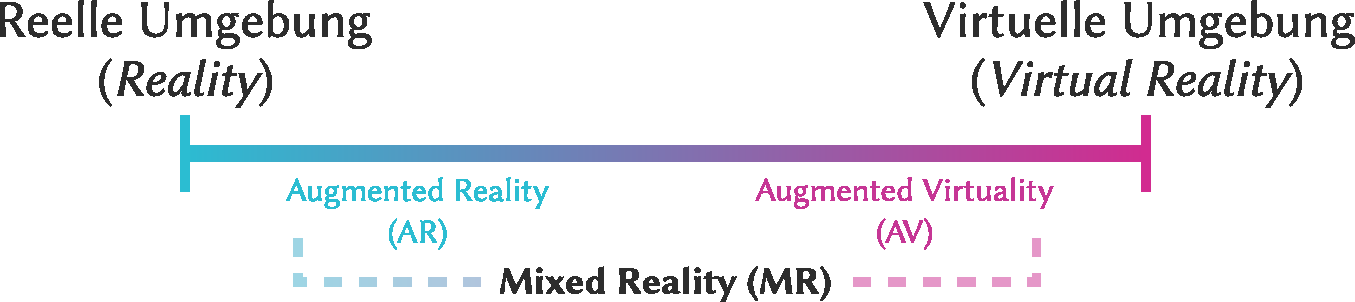
\includegraphics[width=0.9\linewidth]{figures/rv_kontinuum_milgram.pdf}}
    \caption{Das Realität-Virtualität-Kontinuum nach \textcite{Milgram1994}. Je nach Anwendung wird die Realität mehr und mehr mit virtuellen Objekten überlagert, bis schließlich nur noch eine virtuelle Umgebung dargestellt wird.}
    \label{fig:rv_kontinuum}
\end{figure}
Nach \textcite{Azuma1997} bezeichnet \emph{Augmented Reality} Systeme, welche die folgenden Eigenschaften besitzen:
\begin{itemize}
    \item Reale und virtuelle Inhalte werden kombiniert. Häufig werden hierfür virtuelle Objekte auf die reale Umgebung überlagert.
    \item Der Nutzer kann in Echtzeit mit den Systemen interagieren. So zählen z.B. Spezialeffekte in Filmen \emph{nicht} als AR.
    \item Die Inhalte werden dreidimensional mit der Umgebung registriert. Demnach ist ein 2D-Interface vor einer realen Umgebung \emph{kein} AR, selbst wenn es interaktiv ist.
\end{itemize}
AR selbst lässt sich dabei noch in die Kategorien \emph{Spatial AR} und \emph{See-Through AR} einteilen.
Bei Spatial AR werden digitale Informationen direkt in die Umgebung des Nutzers projiziert, z.B. mit einem Projektor auf einen Tisch.
Beim See-Through AR hingegen werden Displays genutzt, die entweder ein Live-Video der Umgebung zeigen oder aber transparent und damit durchsichtig sind.
Dies können See-Through HMDs wie die HoloLens sein, aber auch Smartphones in einer entsprechenden HMD-Halterung, bei denen die Rückseitenkamera für ein Live-Bild der Umgebung genutzt wird.
Hier werden die virtuellen Informationen direkt auf dem Display überlagert \autocite{Zachmann2015}.

Bei der \emph{Augmented Virtuality} (AV) werden umgekehrt reale Informationen in eine virtuelle Umgebung eingebettet.
Als Beispiel nennt \textcite[6]{Schroeder2017} die Wetterkarte im Fernsehen, bei der eine \emph{virtuelle} Karte \emph{reale} Wetterinformationen darstellt und um einen \emph{realen} Moderator erweitert wird.
%Es sei darauf hingewiesen, dass in diesem Beispiel die Interaktion zwischen dem Moderator und der Karte besteht, nicht etwa zwischen dem Zuschauer und der Karte.

\emph{Virtual Reality} ist die Bezeichnung für Anwendungen, die sich komplett in einer virtuellen Umgebung abspielen.
Um VR von herkömmlichen Computersimulationen abzugrenzen nennt \textcite{Zachmann2015} die intuitive Echtzeit-Interaktion als ein wichtiges Kriterium.
Dabei können Nutzer mit der virtuellen Umgebung über Eingabegeräte wie z.B. Controller mit sechs Freiheitsgraden (6DOF) oder haptischen Eingabegeräten interagieren.
Ein weiteres wichtiges Kriterium ist die Immersion.
Diese ergibt sich aus der Summe der vom System stimulierten und gleichzeitig abgeschirmten Sinne.
Aus diesem Grund werden bei VR-Anwendungen häufig HMDs eingesetzt, da diese gleichzeitig den Sehsinn vor der Außenwelt abschirmen und mit virtuellen Bildern stimulieren können.
% TODO: Links zu den Displayarten.
Aber auch halb-immersive Displays wie eine \emph{Cave}, eine \emph{Powerwall} oder ein Volumendisplay sind möglich.

\textcite{Milgram1994} nennen ebenfalls den Begriff der \emph{Mixed Reality} (MR).
Dieser wird in der Literatur als Oberbegriff sowohl für AR als auch AV verwendet.
Der Begriff hebt die Kombination von realen und virtuellen Inhalten hervor.

\section{World-in-Miniature zur Unterstützung der Indoor-Navigation}
% WIM
Die Idee der Megamap ist im Prinzip, ein herunterskaliertes Abbild der Umgebung um den Nutzer zu platzieren.
Damit ist die Megamap eine Variante der World-in-Miniature-Metapher (WIM).
Dies ist ein Ansatz zur Unterstützung von Navigation und Interaktion, der aus dem Bereich der VR stammt.
Dabei wird die nähere Umgebung miniaturisiert dargestellt und häufig als eigenständiges Objekt vom Nutzer in der Hand gehalten.
Je nach Anwendung ergeben sich hieraus unterschiedliche Interaktionsmöglichkeiten \parencite{Stoakley1995}.

\textcites{Mulloni2011a}{Mulloni2012} präsentieren eine See-Through-AR-Anwendung kombiniert aus AR-Hinweisen und WIM.\@
Während Nutzer durch ein Gebäude navigieren werden AR-Pfeile sowie Navigationsanweisungen in Form von \enquote{Aktivitäten} auf einem Smartphone angezeigt (\autoref{sfig:mulloni2011_wim_b}, \subref{sfig:mulloni2011_wim_e}).
Sobald zuvor platzierte Poster an Infopunkten im Gebäude erreicht und gescannt werden, wechselt die Ansicht zu einer WIM-Darstellung der Etage mit der hervorgehobenen Route zum Zielort (\autoref{sfig:mulloni2011_wim_a}, \subref{sfig:mulloni2011_wim_c}, \subref{sfig:mulloni2011_wim_d}).
Die WIM-Übersicht hilft Nutzern, Orientierungspunkte (\emph{\enquote{Landmarks}}) in der Umgebung wiederzuerkennen, was zu weniger Fehlern bei der Navigation führt.
%Von diesem Aspekt könnte auch die Megamap profitieren, welche eine WIM-ähnliche Sicht der näheren Umgebung liefert.
\begin{figure}[t]
    \begin{subfigure}{.18\textwidth}
        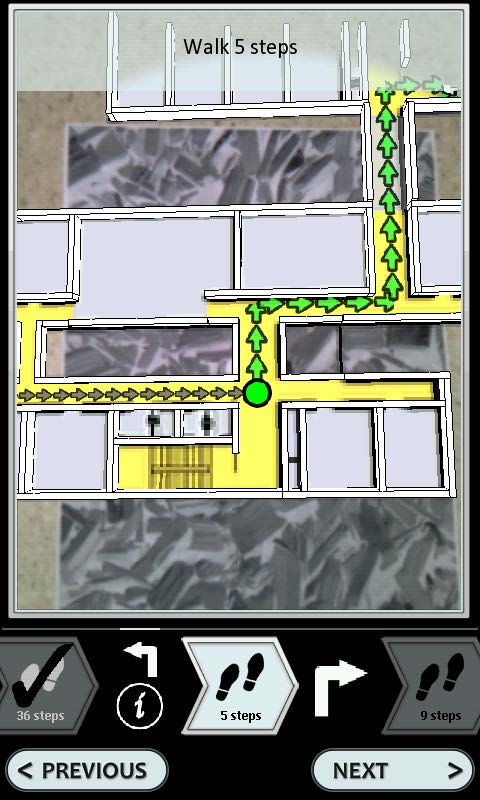
\includegraphics[width=\textwidth]{figures/mulloni2011_wim_a.png}
        \caption{}
        \label{sfig:mulloni2011_wim_a}
    \end{subfigure}
    \hfill
    \begin{subfigure}{.18\textwidth}
        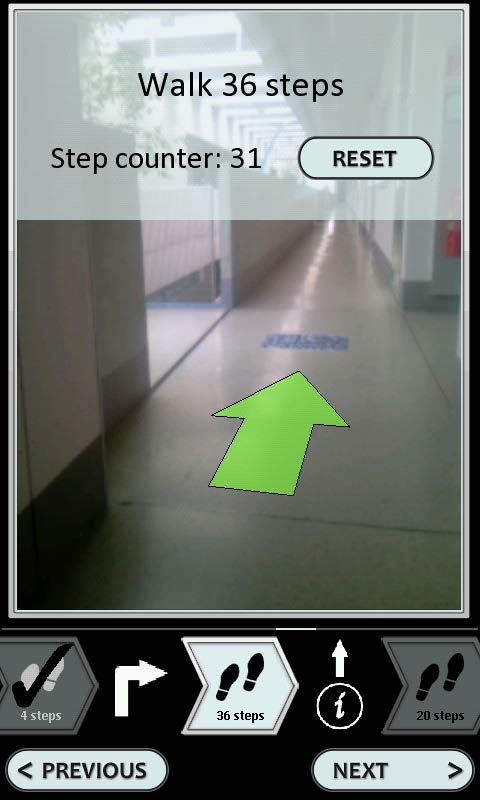
\includegraphics[width=\textwidth]{figures/mulloni2011_wim_b.png}
        \caption{}
        \label{sfig:mulloni2011_wim_b}
    \end{subfigure}
    \hfill
    \begin{subfigure}{.18\textwidth}
        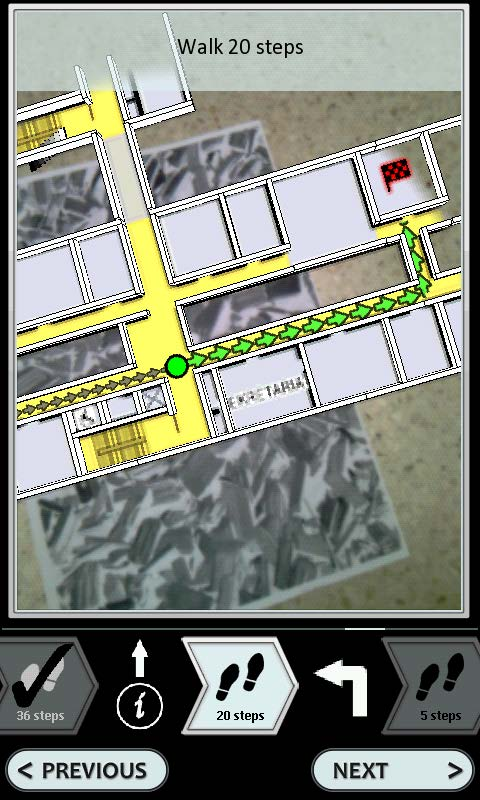
\includegraphics[width=\textwidth]{figures/mulloni2011_wim_c.png}
        \caption{}
        \label{sfig:mulloni2011_wim_c}
    \end{subfigure}
    \hfill
    \begin{subfigure}{.18\textwidth}
        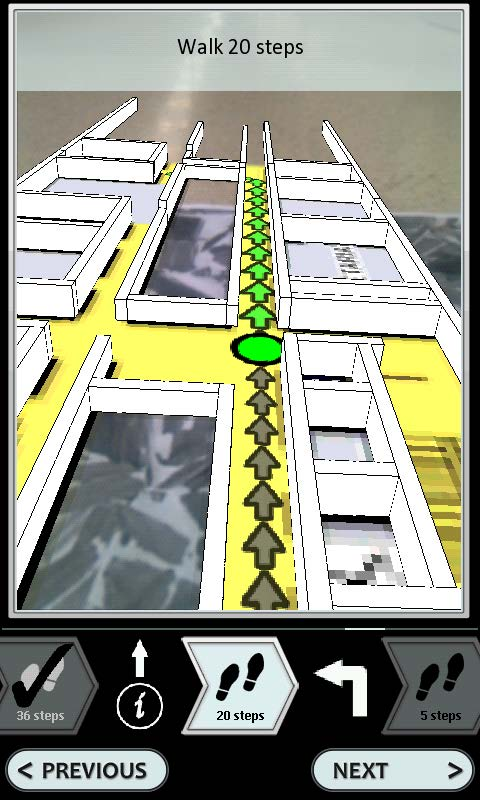
\includegraphics[width=\textwidth]{figures/mulloni2011_wim_d.png}
        \caption{}
        \label{sfig:mulloni2011_wim_d}
    \end{subfigure}
    \hfill
    \begin{subfigure}{.18\textwidth}
        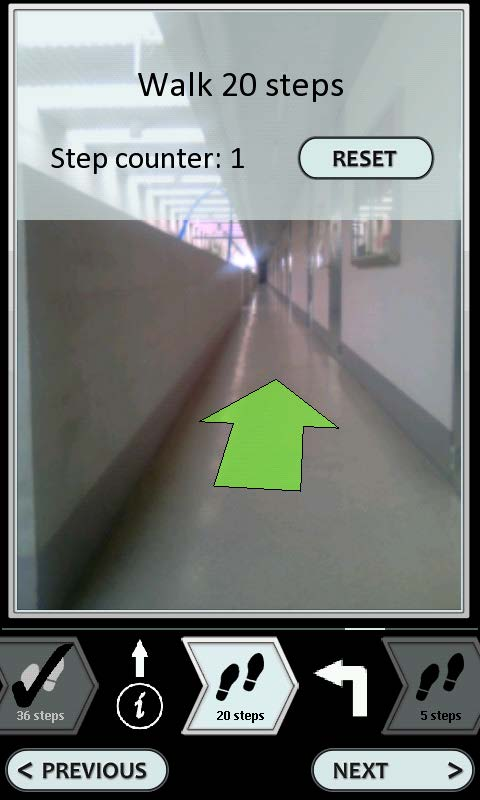
\includegraphics[width=\textwidth]{figures/mulloni2011_wim_e.png}
        \caption{}
        \label{sfig:mulloni2011_wim_e}
    \end{subfigure}
    \quelle{\cite{Mulloni2011}}
    \caption{AR-Interface für Indoor-Navigation basierend auf WIM.\@ An den Lokalisierungspunkten wird die Indoor-Karte als WIM angezeigt und mit der Position/Rotation der Umgebung registriert.}
    \label{fig:mulloni2011_wim}
\end{figure}

Ein Ansatz, welcher der Umsetzung dieser Arbeit nahe kommt, ist die Untersuchung 2D- und 3D-Karten als Navigationshilfe für mehrstöckige Gebäude durch \autocite[siehe \autoref{fig:chittaro2006_maps}]{Chittaro2006}.
Dabei bewegen sich die Nutzer durch ein virtuelles Gebäude von einem Zielobjekt zu einem anderen.
Die Autoren stellen fest, dass für die reine Navigation zwischen zwei Punkten eine 2D-Karte effektiver ist.
Allerdings baut sich die räumliche Vorstellung der Objekte im Gebäude in beiden Darstellungen gleichermaßen auf.
Bei \parencite{Chittaro2006} werden die Karten jedoch von der Umgebung separat dargestellt und die virtuelle Umgebung wird auf einem Nicht-Stereo-Monitor angezeigt.
\begin{figure}[ptb]
	\centering
	\begin{subfigure}{0.6\textwidth}
		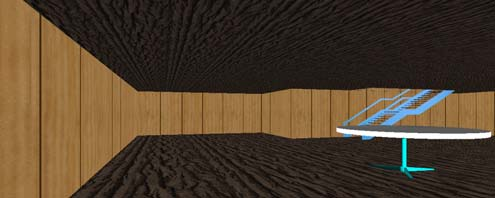
\includegraphics[width=\textwidth]{figures/chittaro2006_ve.png}
		\caption{}
		\label{sfig:chittaro2006_ve}
	\end{subfigure}

	\begin{subfigure}{0.6\textwidth}
		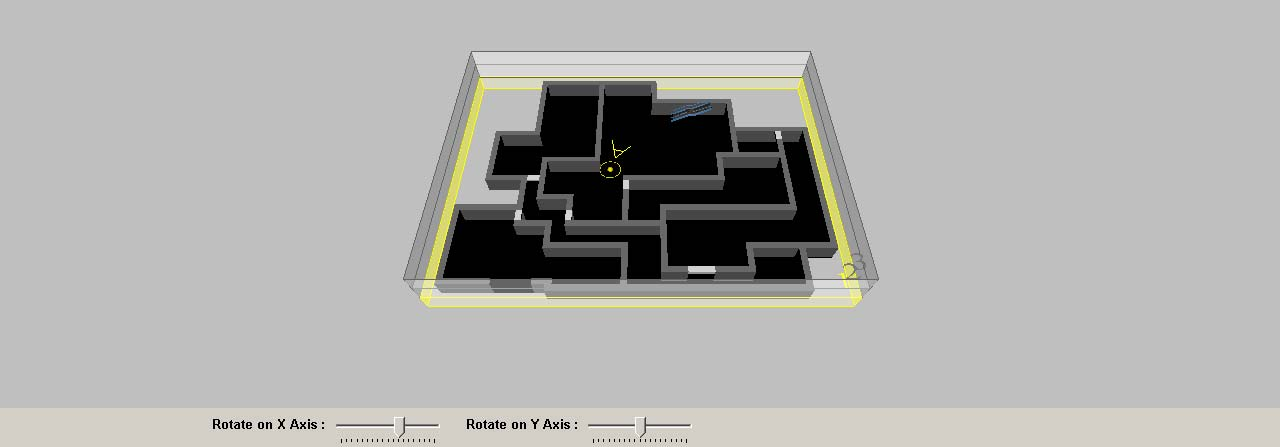
\includegraphics[width=\textwidth]{figures/chittaro2006_3dm.png}
		\caption{}
		\label{sfig:chittaro2006_3dm}
	\end{subfigure}

	\begin{subfigure}{0.6\textwidth}
		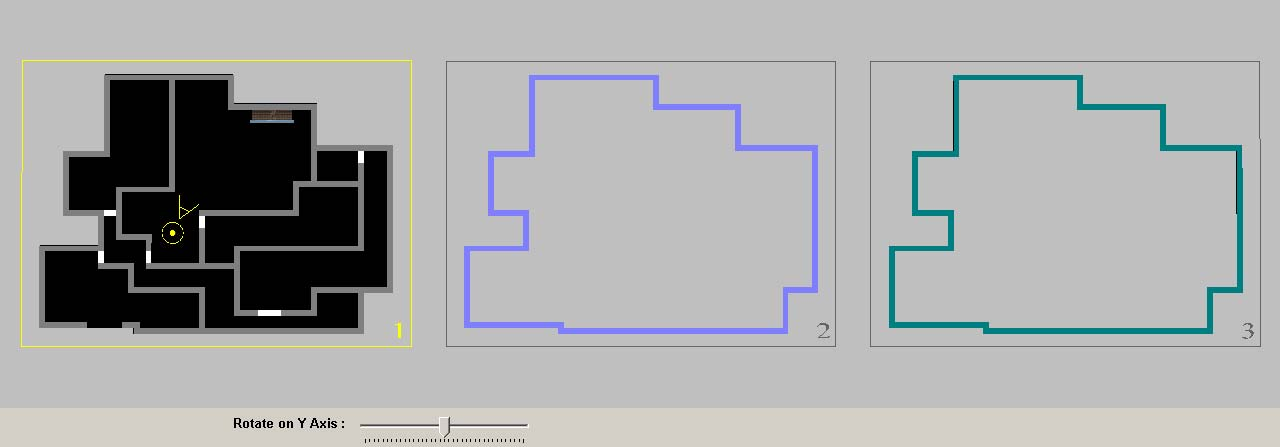
\includegraphics[width=\textwidth]{figures/chittaro2006_2dm.png}
		\caption{}
		\label{sfig:chittaro2006_2dm}
	\end{subfigure}
	\quelle{\cite[230]{Chittaro2006}}
	\caption{Navigation eines virtuellen Gebäudes \subref{sfig:chittaro2006_ve}. Eine 3D-Karte \subref{sfig:chittaro2006_3dm} oder eine 2D-Karte \subref{sfig:chittaro2006_2dm} unterstützen die Navigation.}
	\label{fig:chittaro2006_maps}
\end{figure}

% TODO: Was ist der Mehrwert meiner Arbeit gegenüber dem hier?
In einem früheren Beitrag erweitern \textcite{Chittaro2005} das Konzept von WIM für mehrstöckige Gebäude als eine \emph{BreakAway}-Karte (\autoref{fig:chittaro2005_breakaway}).
Hier können einzelne Stockwerke zur Seite geschoben und ausgeblendet werden, um so auf Stockwerke blicken zu können, auf denen sich der Nutzer selbst gar nicht befindet.
\begin{figure}[ptb]
    \begin{subfigure}{.49\textwidth}
        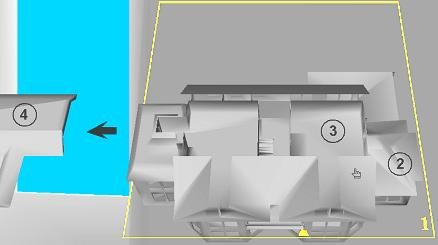
\includegraphics[width=\textwidth]{figures/chittaro2005_breakaway_a.png}
%        \caption{}
    \end{subfigure}
    \hfill
    \begin{subfigure}{.49\textwidth}
        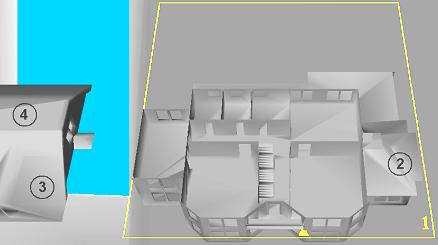
\includegraphics[width=\textwidth]{figures/chittaro2005_breakaway_b.png}
%        \caption{}
    \end{subfigure}
    \quelle{\cite{Chittaro2005}}
    \caption{In der \emph{\enquote{Examine View}} der BreakAway-Karte können Stockwerke zur Seite geschoben werden, um den Blick auf darunterliegende Stockwerke zu ermöglichen.}
    \label{fig:chittaro2005_breakaway}
\end{figure}
\textcite{Vallance2001} schlagen zudem eine Krümmung der WIM-Umgebung vor, um so ein Verdecken durch Wände und andere Objekte zu minimieren.

% TODO: Weiter ausführen?
Auch \textcite{Li2013} untersuchen die Auswirkungen von 2D- und 3D-Dar\-stel\-lun\-gen von mehrstöckigen Gebäuden.
Satt einer detaillierten Karte wird hier nur eine strukturelle Karte (Flur und Treppen) gezeigt.
Im Fall der 3D-Karte rotiert die Ansicht automatisch, wenn die Nutzer sich bewegen.
Das Ergebnis der Autoren ist, dass sich beide Darstellungen gleichermaßen zum Aufbau eines räumlichen Verständnisses des Gebäudes eignen.
Allerdings wurden hier nur zweistöckige Gebäude getestet.
Für diese Arbeit ist jedoch auch die Skalierung auf Gebäude mit mehr Stockwerken interessant.

\section{Virtuelle Navigationshelfer}
Bereits \textcite{Hoellerer1999} stellen ein AR-System vor, bei dem zwei Nutzer kooperieren können.
Der eine Nutzer bewegt sich zu Fuß mit einem HMD und einem Tablet-Computer in der Außenwelt.
Durch das HMD können ihm augmentierte Informationen zur Umgebung und sogar ganze virtuelle Gebäude dargestellt werden, die mit der Umgebung registriert sind.
Der andere Nutzer kann entweder über ein Desktop-Interface oder eine AR-Darstellung der Karte Routen und Informationen in der Umgebung platzieren.
Damit stellt diese Arbeit eine frühe Implementierung für ein HMD dar, die sowohl Navigations- als auch Explorationsaufgaben unterstützt.

Wie bereits in \autoref{sec:motivation_ziel} erwähnt fokussiert sich ein großer Teil der bisherigen Forschung auf den Usecase der Navigation von einem Punkt zu einem anderen.
Vor allem das AR-unterstützte Autofahren wird betrachtet, da hier eine fehlerfreie Navigation wichtig ist und im Fehlerfall sogar fatale Folgen haben kann \parencite{Lin2017}.
Ein häufig eingesetztes Mittel ist hier die virtuelle Hervorhebung der Straßenführung.
\textcite{Narzt2006} präsentieren ein allgemeines Framework zur Darstellung einer virtuellen Route.
Das Framwork kann sowohl für Fahrzeug- als auch Fußgängernavigation und auf verschiedenen Endgeräten eingesetzt werden.
Für den Einsatz im Auto schlagen die Autoren die Windschutzscheibe als Display vor.
Dadurch wäre das AR-Display in der natürlichen Umgebung des Nutzers integriert.
\textcite{Bark2014} erweitern diesen Ansatz.
Sie ersetzen in einem zuvor aufgenommenen Video die statische virtuelle Route durch eine Reihe animierter Papierflieger, die entlang der geplanten Route fliegen.
\textcite{Kim2009} ersetzen die Route sogar durch eine 2.5D-Karte mithilfe eines Fahrsimulators.
Von der Oberseite der Windschutzscheibe schiebt sich eine 2D-Karte ins Sichtfeld, die sich nach und nach dreidimensional mit der Straße verbindet.
Bei beiden Ansätzen wiesen die Autoren beim Vergleich mit einem herkömmlichen \emph{top-down} GPS-System nach, dass die Probanden dem Straßenverlauf durch die AR-Unterstützung besser folgen konnten und weniger Fehler bei der Navigation machten.

\textcite{Alnabhan2014} präsentieren einen Ansatz zur \emph{Indoor}-Navigation als \emph{Android-App}.
Die App nutzt \emph{\wifi-Fingerprinting} und den digitalen Kompass eines Smartphones/Tablets zur Positionierung und Orientierung.
Über vordefinierte Referenzpunkte im Gebäude wird die Ungenauigkeit des \wifi-Fingerprintings ausgeglichen.
Navigationshinweise werden als AR-Pfeil angezeigt (mit zusätzlichen Textausgaben).
Alternativ dazu zeigen \textcite{Liu2016} einen ähnlichen Ansatz, bei dem die Positionierung jedoch auf Magnetfeldsensoren aufbaut und daher weder auf GPS noch auf Infrastruktur wie \wifi oder Marker angewiesen ist.

\section{Augmentierte Kartenexploration}
Zur Kartenexploration mittels Spatial AR tragen \textcite{Reitmayr2005} bei, indem sie eine reale Papierkarte durch einen Projektor augmentieren.
\autoref{fig:reitmayr2005_helicopter_map} zeigt die Funktionsweise.
Ein projizierter Helikopter kann mit einem realen \emph{Personal Digital Assistant} (PDA) bewegt werden, wenn dieser in die Nähe gehalten wird.
Der PDA zeigt währenddessen ein Interface zur Kontrolle des Helikopters.
Der Helikopter dient als Cursor für kontextbasierte Informationen.
Sobald der Nutzer einen Rahmen auf die Karte legt, projiziert der Projektor ein Bild der aktuellen Kartenposition aus ungefährer Sicht des Helikopters auf ihn.
Zudem kann der Zustand der Karte durch die Projektion dynamisch verändert werden (in diesem Fall werden Gezeiten von Gewässern simuliert).
Auch wenn diese Arbeit nicht für einen mobilen Einsatz geeignet ist, wird deutlich, dass mit AR nicht nur ortsbezogene sondern auch zeitbezogene Daten auf einer Karte dargestellt werden können.
Dies erlaubt also zusätzlich eine Exploration in der zeitlichen Dimension einer Karte.
\begin{figure}
    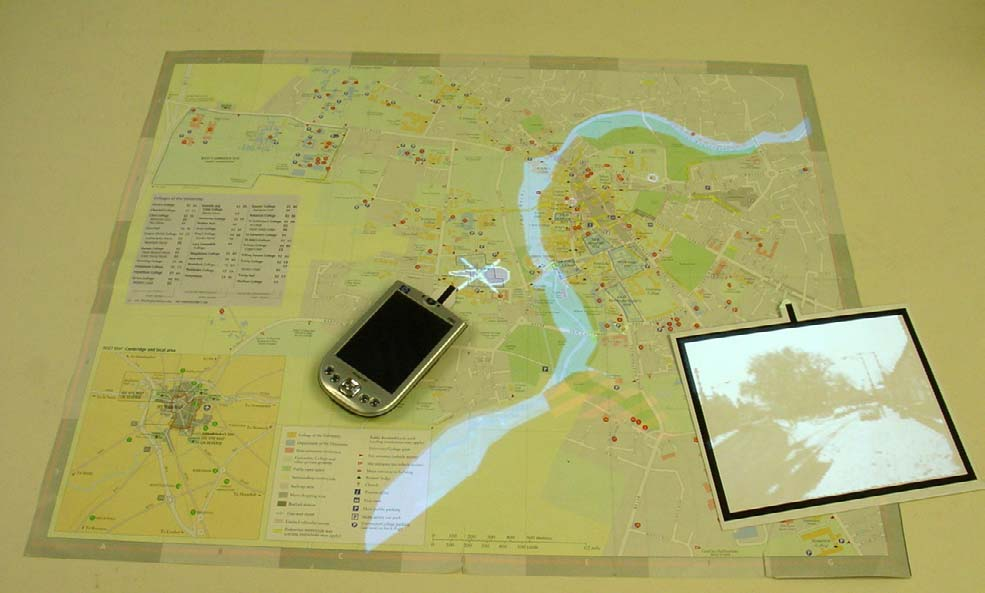
\includegraphics[width=\textwidth]{figures/reitmayr2005_helicopter_map.png}
    \quelle{\cite{Reitmayr2005}}
    \caption{Eine reale Papierkarte wird durch einen Projektor mit virtuellen Inhalten angereichert.}
    \label{fig:reitmayr2005_helicopter_map}
\end{figure}

\section{Navigation und Exploration in digitalen Spielen}
Wie in \autoref{sec:motivation_ziel} erwähnt nehmen Navigation und Exploration eine wichtige Rolle in digitalen Spielen ein.
Daher finden sich zu diesen Themen verschiedene Herangehensweisen.

Im Bereich der Video- und Computerspiele untersuchen \textcites{Moura2014}{Moura2015} den Zusammenhang zwischen eingesetzten Navigationshelfern, Design der Level, sowie Spielmechaniken zur Unterstützung der Navigation.
Daraus leiten \textcite{Moura2015} eine Klassifikation von Navigationshelfern ab.
Außerdem erstellen sie eine Liste von Design-Richtlinien, welche die Vor- und Nachteile der jeweiligen Helfer erläutern und als Hilfestellung für Entwicklung von neuen Spielen dienen.
Diese Designrichtlinien werden in die Entwicklung der Megamap mit einbezogen.

Aufbauend auf die Navigationshelfer in Spielen untersucht \textcite{Lodts2015}, ob diese Helfer auch in der realen Welt anwendbar sind.
Dazu wurden unterschiedliche Helfer, wie sie aus Spielen bekannt sind, für das \emph{Google Glass} implementiert.
In einem Test, aufgeteilt in die Aufgabenbereiche Navigation, Orientierung, Exploration und Annotation, wurde ermittelt welche der Helfer den Nutzern bei der jeweiligen Aufgabe am hilfreichsten sind.
Es zeigt sich, dass Helfer, die in der Umgebung eingebettet sind (z.B. AR-Pfeile oder -Text, farbliche Hervorhebungen von Objekten) effektiver sind als statische Anzeigen per \emph{Head-Up Display} (HUD).
Daher wird bei der Entwicklung der Megamap-Anwendung der AR-Darstellung von Inhalten mehr Beachtung geschenkt.

\section{Beitrag dieser Masterarbeit}
Diese Arbeit hebt sich in zwei Aspekten vom bisherigen Stand der Forschung ab.
Zum einen wird eine Kartenanwendung speziell für ein VR-HMD entwickelt.
Dadurch kann die Karte direkt in die (virtuelle) Umgebung des Nutzer eingebettet werden.
Die Verwendung des Stereodisplays im HMD erweitert die Tiefenwahrnehmung der Nutzer, was für die Betrachtung der komplexen mehrstöckigen Innenstrukturen von Gebäuden hilfreich ist. % TODO: Ist das so?
Die Implementierung für ein VR-HMD kann als Sprungbrett für zukünftige Arbeiten betrachtet werden, die das gleiche Konzept für MR-HMDs umsetzen könnten, bei denen die Karte in die \emph{reale} Umgebung des Nutzers integriert wird (siehe \autoref{chap:closing}).

Zum anderen wird der Anwendungsfall der Indoor-Kartenexploration näher beleuchtet.
Wie zu sehen ist setzen sich die bisherigen Ansätze im Bezug auf Indoor-Orte meistens nur mit der reinen Navigation auseinander oder Lokalisierung auseinander.
Diese Arbeit fokussiert hingegen die Kartenexploration.
Zu diesem Zweck wird unter anderem analysiert, wie bereits existierende Kartenanwendungen den Nutzern das Erkunden ihrer Umgebung vereinfachen.
Dabei beschränkt sich die Analyse nicht nur auf Indoor-Anwendungen, sondern bezieht auch Outdoor-Anwendungen (z.B. Google Maps) oder gar digitale Spiele mit ein.
Schließlich werden die hieraus gewonnenen Erkenntnisse auf den Indoor-Einsatz übertragen und prototypisch implementiert.
%
\cleardoublepage
